%%%%%%%%%%%%%%%%%%%%%%%%%%%%%%%%%%%%%%%%%
% Formal Book Title Page
% LaTeX Template
% Version 2.0 (23/7/17)
%
% This template was downloaded from:
% http://www.LaTeXTemplates.com
%
% Original author:
% Peter Wilson (herries.press@earthlink.net) with modifications by:
% Vel (vel@latextemplates.com)
%
% License:
% CC BY-NC-SA 3.0 (http://creativecommons.org/licenses/by-nc-sa/3.0/)
%
% This template can be used in one of two ways:
%
% 1) Content can be added at the end of this file just before the \end{document}
% to use this title page as the starting point for your document.
%
% 2) Alternatively, if you already have a document which you wish to add this
% title page to, copy everything between the \begin{document} and
% \end{document} and paste it where you would like the title page in your
% document. You will then need to insert the packages and document
% configurations into your document carefully making sure you are not loading
% the same package twice and that there are no clashes.
%
%%%%%%%%%%%%%%%%%%%%%%%%%%%%%%%%%%%%%%%%%

%----------------------------------------------------------------------------------------
% PACKAGES AND OTHER DOCUMENT CONFIGURATIONS
%----------------------------------------------------------------------------------------

\documentclass[a4paper, 11pt, oneside]{book} % A4 paper size, default 11pt font size and oneside for equal margins

\newcommand{\plogo}{\fbox{$\mathcal{PL}$}} % Generic dummy publisher logo

\usepackage[utf8]{inputenc} % Required for inputting international characters
\usepackage[T1]{fontenc} % Output font encoding for international characters
\usepackage{fouriernc} % Use the New Century Schoolbook font
\usepackage{hyperref}
\usepackage{geometry}
\geometry{
	a4paper,
	total={170mm,257mm},
	left=25mm,
	top=20mm,
}
\usepackage{graphicx}
\graphicspath{ {.} }
\usepackage{caption}

\usepackage{calc}

\usepackage{mdframed}
\usepackage{fancybox}

%----------------------------------------------------------------------------------------
% TITLE PAGE
%----------------------------------------------------------------------------------------



\begin{document}

\begin{titlepage} % Suppresses headers and footers on the title page

 \centering % Centre everything on the title page

 \scshape % Use small caps for all text on the title page

 \vspace*{\baselineskip} % White space at the top of the page

 %------------------------------------------------
 % Title
 %------------------------------------------------

 \rule{\textwidth}{1.6pt}\vspace*{-\baselineskip}\vspace*{2pt} % Thick horizontal rule
 \rule{\textwidth}{0.4pt} % Thin horizontal rule

 \vspace{0.75\baselineskip} % Whitespace above the title

 {\LARGE Welcome To Anypoint Platform Architecture: \\
 		Application Networks \\ \small\LaTeX ~} % Title

 \vspace{0.75\baselineskip} % Whitespace below the title

 \rule{\textwidth}{0.4pt}\vspace*{-\baselineskip}\vspace{3.2pt} % Thin horizontal rule
 \rule{\textwidth}{1.6pt} % Thick horizontal rule

 \vspace{2\baselineskip} % Whitespace after the title block

 %------------------------------------------------
 % Subtitle
 %------------------------------------------------

 % Subtitle or further description

 \vspace*{3\baselineskip} % Whitespace under the subtitle

 %------------------------------------------------
 % Editor(s)
 %------------------------------------------------

 Edited By

 \vspace{0.5\baselineskip} % Whitespace before the editors

 {\scshape\Large Boyuan Zhang \\} % Editor list

 \vspace{0.5\baselineskip} % Whitespace below the editor list

 \textit{} % Editor affiliation

 \vfill % Whitespace between editor names and publisher logo

 %------------------------------------------------
 % Publisher
 %------------------------------------------------

 %\plogo % Publisher logo

 \vspace{0.3\baselineskip} % Whitespace under the publisher logo

 2019 % Publication year

  {\large } % Publisher

\end{titlepage}

%----------------------------------------------------------------------------------------

\newpage




\tableofcontents

%\part{Week 1}

\chapter{Introduction}

\section{Integration architecture and Platform architecture}

\begin{itemize}

	\item Anypoint Platform Architecture: \textbf{Application Networks} and MuleSoft Certified \textbf{Platform Architect} - Level 1

	\begin{itemize}
		\item Define and be responsible for an organization's Anypoint Platform strategy
		\item Direct the emergence of an effective application network out of individual integration solutions following API-led connectivity across an organization
	\end{itemize}

	\item Anypoint Platform Architecture: \textbf{Integration Solutions} and MuleSoft Certified \textbf{Integration Architect} - Level 1

	\begin{itemize}
		\item Drive and be responsible for an organization's Anypoint Platform implementation and the technical quality, governance (ensuring compliance), and operationalization of the integration solutions.
		\item Work with technical and non-technical stakeholders to translate functional and non-functional requirements into integration interfaces and implementations
	\end{itemize}

\end{itemize}

\section{Prerequisites for Anypoint Platform architecture}

\textbf{Experience with Anypoint Platform} and its constituent components

\begin{itemize}
	\item \textit{Getting Started} with \textit{Anypoint Platform}
	\item \textit{Anypoint Platform Development}: Fundamentals
	\item \textit{MuleSoft.U development Fundamentals}
	\item \textit{API-Led connectivity Workshop} by MuleSoft Presales upon request
\end{itemize}

\begin{mdframed}[backgroundcolor=yellow]
	The \textit{target audience} of this course are architects, especially Enterprise Architects and Solution Architects, new to Anypoint Platform, API-led connectivity and the application network approach, but experienced in other
\end{mdframed}


\section{Goals}

\begin{itemize}
	\item \textbf{Direct} the emergece of an effective \textbf{application network} out of individual integration solutions following API-led connectivity, working \textbf{with all relevant stakeholders} on all levels of the organization
	\item \textbf{Create} credible \textbf{high-level architecture models} for integration solutions on Anypoint Platform such that functional and non-functional requirements are likely to be met and the principles of \textbf{API-led connectivity} and application networks are followed 
	\item Predominantly about \textbf{cloud-native architectures} using the MuleSoft-hosted Anypoint Platform, i.e. \textbf{CloudHub} 
\end{itemize}

\section{Outline}

\begin{enumerate}
	\item Putting the Course in Context
	\item Introducing MuleSoft, the Application Network Vision and Anypoint Platform
	\item Establishing Organizational and Platform Foundations
	\item Identifying, Reusing and Publishing APIs
	\item Enforcing NFRs on the Level of API Invocations Using Anypoint API Manager
	\item Designing Effective APIs
	\item Architecture design and Deploying Effective API Implementations
	\item Augmenting API-Led Connectivity with Elements From Event-Driven Architecture
	\item Transiting Into Production
	\item Monitoring and Analyzing the Behavior of the application Network  
\end{enumerate}

\begin{figure}[h]
	
	\begin{minipage}{1\textwidth}
		\centering
		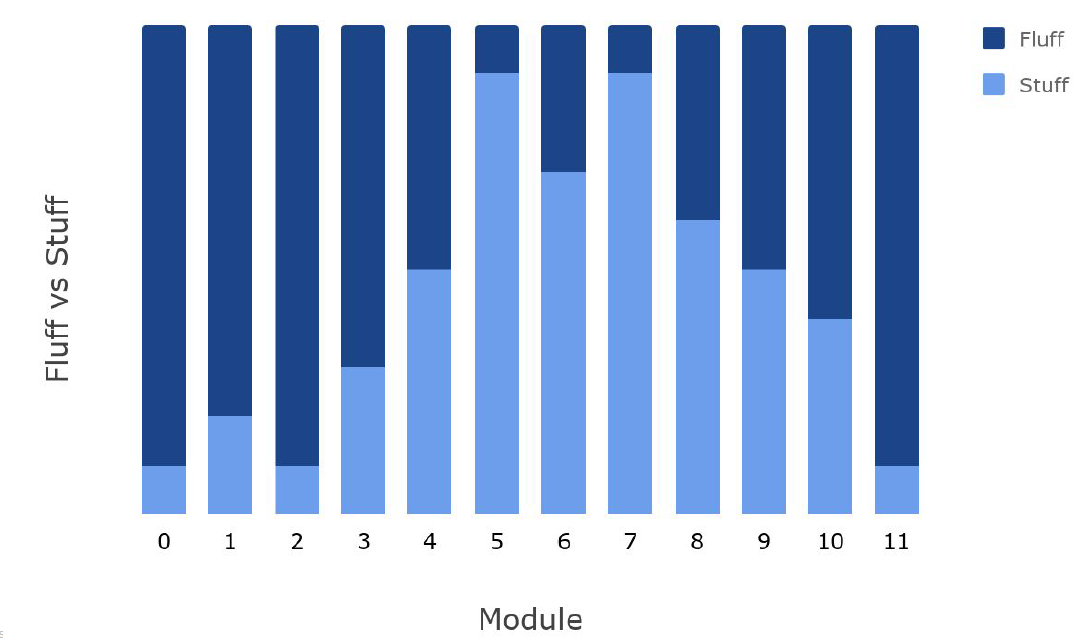
\includegraphics[width=1\linewidth]{FluffAndStuff}
		%\caption{No eavesdropping no tampering}\label{}
	\end{minipage}
	
\end{figure}

\section{How the course will work}

\begin{itemize}
	\item Central topic: How to \textbf{architect and design application networks} using API-led connectivity and Anypoint Platform. (Partly \textbf{Solution Architecture}, partly \textbf{Enterprise Architecture})
	\item No architecturally \textbf{insignificant} design and implementation discussion
	(Fairly detailed discussion on strategies for invoking APIs in a fault-tolerant way)
	\item RAML features are touched-on because they are important for the functioning of an application network
\end{itemize}

\begin{mdframed}[backgroundcolor=yellow]
	
	\begin{itemize}
		\item Discussions on topics like scale of Enterprise Architecture, touching lightly on Business Architecture, and heavily on Application Architecture and Technology Architecture.
		\item Motivations and Enterprise Architecture Building from strategically important integration solutions and therefore elaborates on parts of their high-level Solution Architecture. 
		\item It stays away from architecturally insignificant design and implementation discussions: 
		\begin{itemize}
			\item As a rule, these are all topics whose repercussions are confined to individual application components and are therefore not apparent from outside these application components. 
			\item When a decision affects the large-scale properties of the application network, however, it becomes architecturally significant. This is the reason why the course contains a fairly detailed discussion on strategies for invoking APIs in a fault-tolerant way
			\item The topic of API specifications and the features offered by RAML in this space are touched upon in several places, because they are important for the functioning of an application network.
		\end{itemize}	
	\end{itemize}
	
	This course is primarily driven by a single \textit{case study}, \textit{Acme Insurance}, and two imminent strategically important change initiatives that need to be addressed by Acme Insurance. These change initiative provide the background and motivation for most discussions in this course.
	
	As various aspects of the case study are addressed, the discussion naturally elaborates on the central topic of the course, i.e., \textit{how to architect and design application networks using API-led connectivity and Anypoint Platform}.
	
\end{mdframed}

\end{document}
